\documentclass{article}
\usepackage{main}

\author{Maths Spécifiques}
\date{4 Mars 2024}
\title{Modèles affines}

\begin{document}
\maketitle

La figure suivante montre l'évolution du niveau moyen des océans mesuré
entre 1993 et 2019. Le niveau constaté en 1993 est pris comme référence et
fixé à 0 cm.

\begin{center}
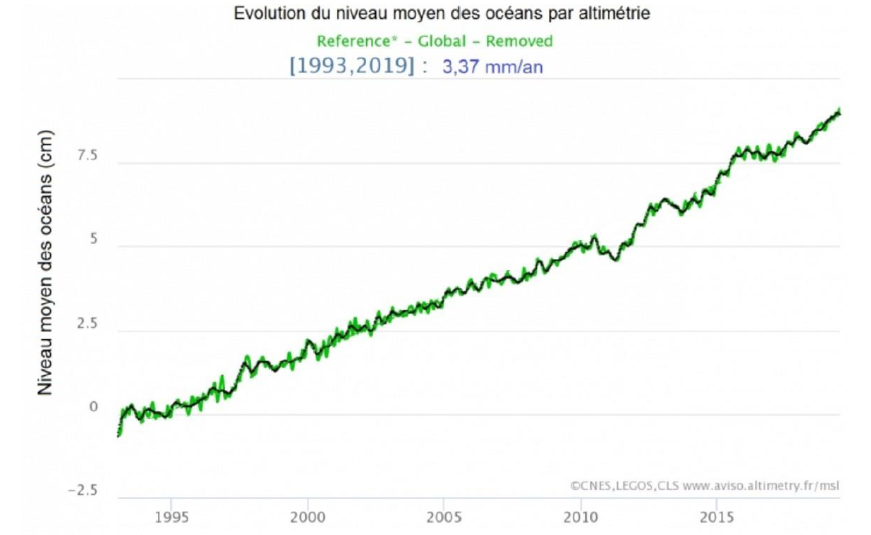
\includegraphics[scale=0.6]{NiveauOcean.png}
\end{center}
\section{Modélisation}
\begin{enumerate}
\item Quel est le niveau moyen des océans en 2000 ? Et en 2010 ?
\item Quelle est la tendance générale décrite par la courbe ? Par quelle valeur donnée dans la figure cette tendance se traduit-elle ?
\item Si la tendance se poursuit, quel sera le niveau moyen des océans d'ici 2030 ? 
\end{enumerate}
Pour illustrer cette tendance générale, nous allons utiliser un \emph{modèle affine}. Cela correspond à une droite dont les points sont proches des points de la courbe. Pour tracer une telle droite, il suffit de prendre deux points aux \og extremités \fg de la courbe représentée.
\begin{enumerate}[resume*]
\item Essayez de tracer à la règle une telle droite sur votre figure.
\item Quelle est sa pente ? Le justifier en utilisant la formule de la variation entre ordonnées et abscisses.
\end{enumerate}

\section{Prévisions}
Maintenant que nous avons un modèle traduisant la tendance générale, nous pouvons effectuer des prévisions.
\begin{enumerate}[resume*]
\item Donner l'expression de la fonction affine dont la courbe représentative est la droite que vous avez construite.
\item En déduire un niveau moyen des océans hypothétique en $2030$.
\item Même question en $2050$.
\end{enumerate}
\section{Pertinence du modèle}
Discutez la pertinence du modèle : tracer une telle droite vous semnle-t-il adapté à modéliser tous les phénomènes ?

Voici la courbe illustrant la température :
\begin{center}
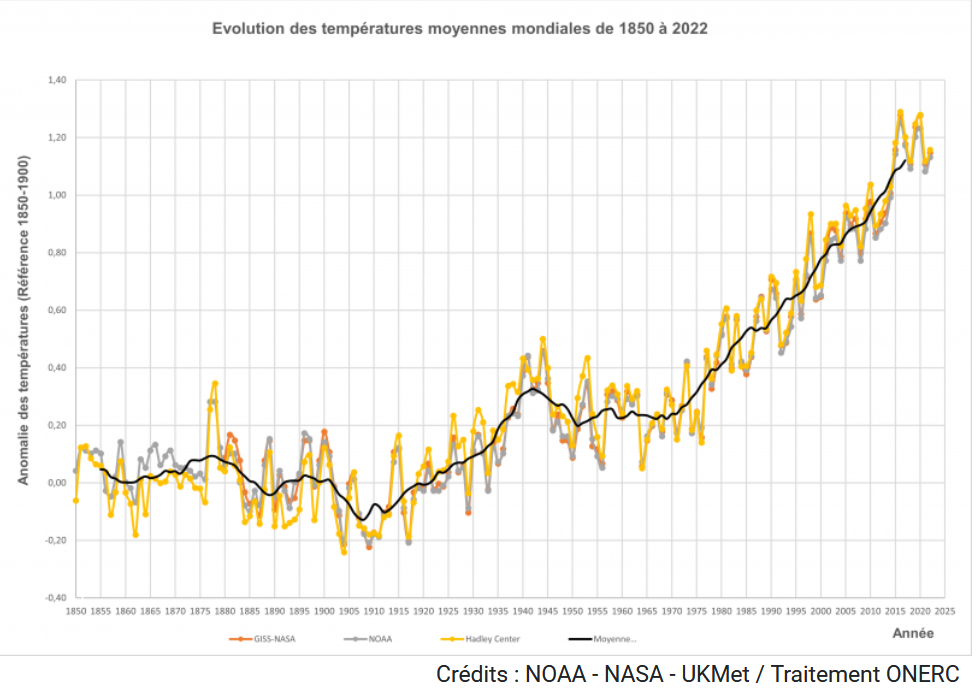
\includegraphics[scale=0.6]{Temperatures.png} 
\end{center}

Le modèle affine est-il pertinent ici pour établir des projections ? 
\end{document}